\section{Descrizione Testuale strutturata del Sistema}
In questa sezione faremo un analisi più approfondita di alcuni dei casi d'uso campione del sistema, per esporre il nostro ragionamento per modellare e sviluppare il Software .\\
Questa descrizione ci servirà per pensare a che tipo di interazioni con l'Utente sono necessarie, i passaggi da effettuare  dal sistema in risposta alle richieste ricevute e 
I casi d'uso scelti per questo scopo sono la Creazione di un nuovo Annuncio di un Immobile e Modifica notifiche in Arrivo.
  
\subsection{Cockburn: nuovo annuncio}

\begin{figure}[H]
	\centering
	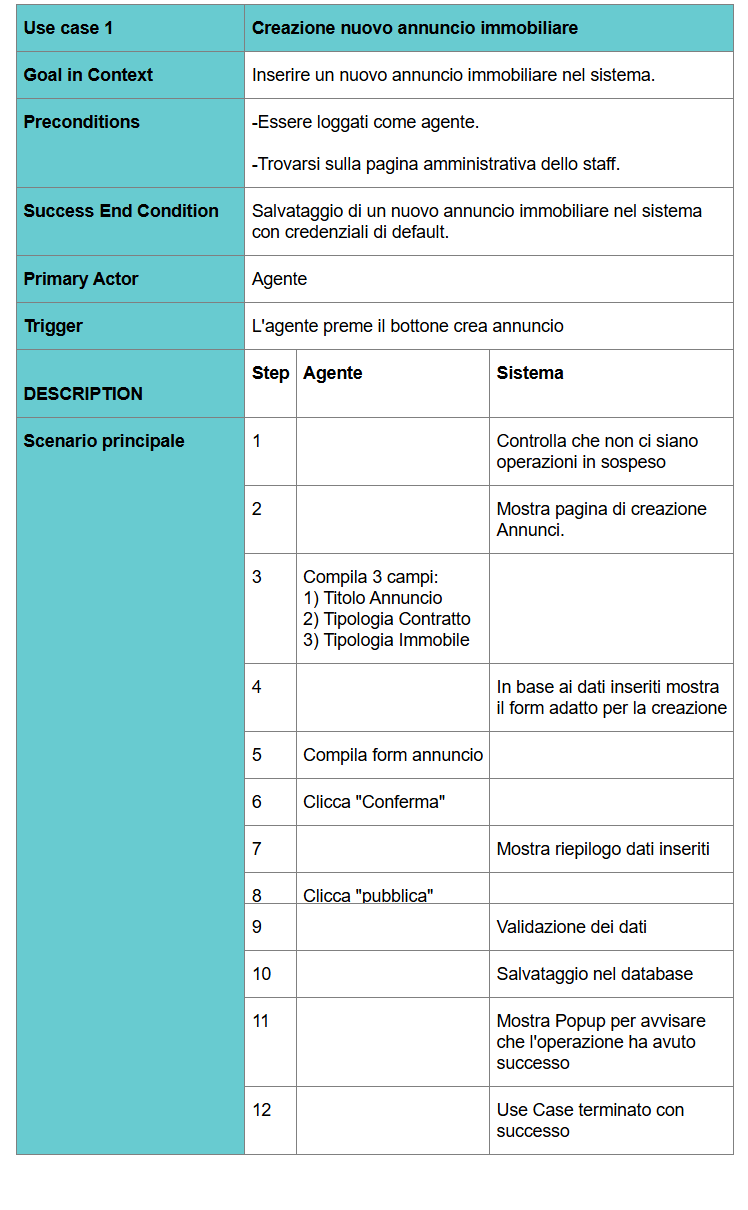
\includegraphics[width=1\linewidth]{"Immagini/cockburn/nuovo annuncio principale.png"}
	\caption[CockBurn extensions: registra nuovo annuncio]{}
	\label{fig:registra-nuovo-annuncio-principale}
\end{figure}

\newpage

\begin{figure}[H]
	\centering
	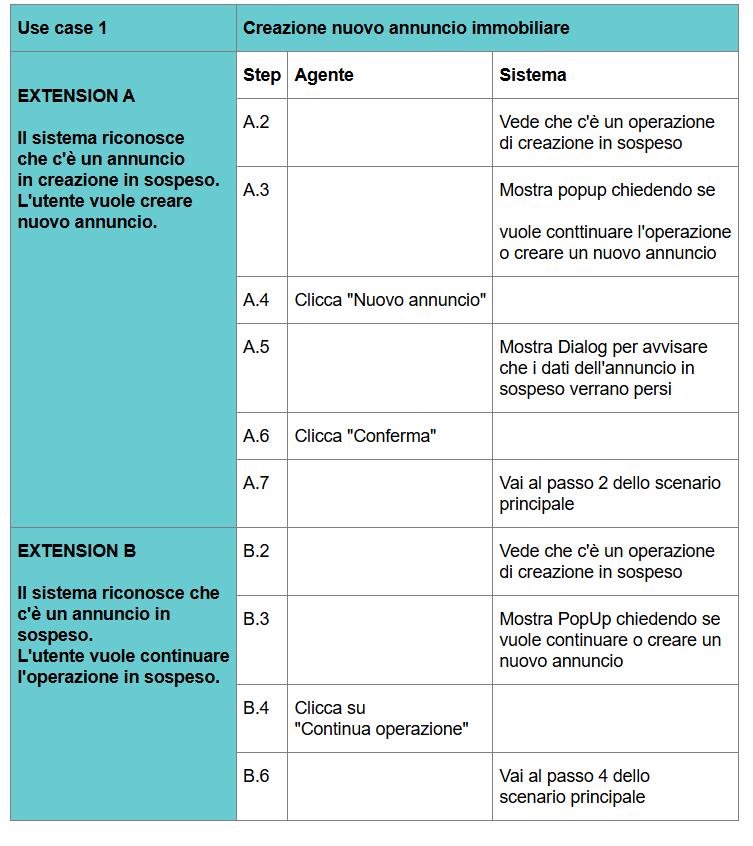
\includegraphics[width=1\linewidth]{"Immagini/cockburn/nuovo annuncio estensioni 1.png"}
	\caption[CockBurn extensions: registra nuovo annuncio]{}
	\label{fig:registra-nuovo-annuncio-extensions1}
\end{figure}

\newpage

\begin{figure}[H]
	\centering
	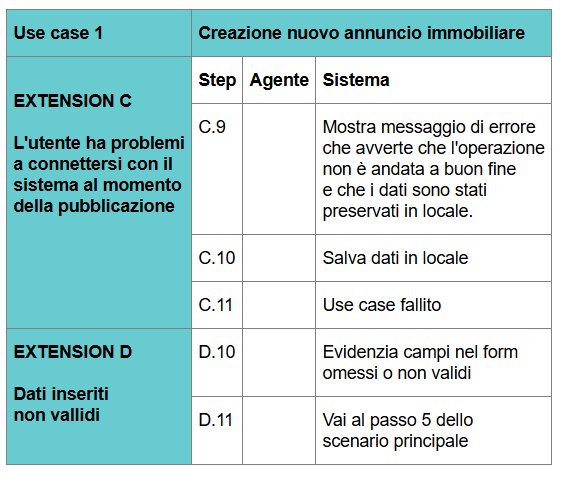
\includegraphics[width=1\linewidth]{"Immagini/cockburn/nuovo annuncio estensioni 2.png"}
	\caption[CockBurn extensions: registra nuovo annuncio]{}
	\label{fig:registra-nuovo-annuncio-extensions2}
\end{figure}
\newpage
% Please add the following required packages to your document preamble:
% \usepackage{multirow}
% \usepackage[table,xcdraw]{xcolor}
% Beamer presentation requires \usepackage{colortbl} instead of \usepackage[table,xcdraw]{xcolor}
% \usepackage{longtable}
% Note: It may be necessary to compile the document several times to get a multi-page table to line up properly
\begin{longtable}{|l|lll|}
\caption{}
\label{tab:my-table}\\
\hline
\rowcolor[HTML]{E1D5E7} 
\textbf{Use Case 2}                                                                                                                                                                 & \multicolumn{3}{l|}{\cellcolor[HTML]{E1D5E7}\textbf{Modifica notifiche in Arrivo}}                                                                                                                                                                                                                                                                                                                        \\ \hline
\endhead
%
\cellcolor[HTML]{E1D5E7}\textbf{Goal In Context}                                                                                                                                    & \multicolumn{3}{l|}{Cambia lo stato di notiche a scelta}                                                                                                                                                                                                                                                                                                                                                  \\ \hline
\cellcolor[HTML]{E1D5E7}\textbf{Preconditions}                                                                                                                                      & \multicolumn{3}{l|}{\begin{tabular}[c]{@{}l@{}}- Login effettuato con account con\\ ruolo Utente. \\ - Si trova nella pagina di Visualizazione notifiche\end{tabular}}                                                                                                                                                                                                                                    \\ \hline
\cellcolor[HTML]{E1D5E7}\textbf{\begin{tabular}[c]{@{}l@{}}Success End\\ Conditions\end{tabular}}                                                                                   & \multicolumn{3}{l|}{Lo stato di abilitazione di notifica viene modificato}                                                                                                                                                                                                                                                                                                                                \\ \hline
\cellcolor[HTML]{E1D5E7}\textbf{Primary Actor}                                                                                                                                      & \multicolumn{3}{l|}{Utente}                                                                                                                                                                                                                                                                                                                                                                               \\ \hline
\cellcolor[HTML]{E1D5E7}\textbf{Trigger}                                                                                                                                            & \multicolumn{3}{l|}{Utente preme il bottone Gestisci Notifiche}                                                                                                                                                                                                                                                                                                                                           \\ \hline
\rowcolor[HTML]{E1D5E7} 
\textbf{Descrizione}                                                                                                                                                                & \multicolumn{1}{l|}{\cellcolor[HTML]{E1D5E7}\textbf{Step n.}} & \multicolumn{1}{l|}{\cellcolor[HTML]{E1D5E7}\textbf{Utente}}                                                                            & \textbf{Sistema}                                                                                                                                                                                \\ \hline
\cellcolor[HTML]{E1D5E7}                                                                                                                                                            & \multicolumn{1}{l|}{1}                                        & \multicolumn{1}{l|}{}                                                                                                                   & \textit{\begin{tabular}[c]{@{}l@{}}Mostra pagina delle\\ notifiche\end{tabular}}                                                                                                                \\ \cline{2-4} 
\cellcolor[HTML]{E1D5E7}                                                                                                                                                            & \multicolumn{1}{l|}{2}                                        & \multicolumn{1}{l|}{\begin{tabular}[c]{@{}l@{}}Click Bottone per\\ modificare stato notifica\end{tabular}}                              &                                                                                                                                                                                                 \\ \cline{2-4} 
\cellcolor[HTML]{E1D5E7}                                                                                                                                                            & \multicolumn{1}{l|}{3}                                        & \multicolumn{1}{l|}{}                                                                                                                   & \textit{\begin{tabular}[c]{@{}l@{}}Mosta una Popup con \\ elenco di tutte le \\ categorie che possono \\ essere Modificate\end{tabular}}                                                        \\ \cline{2-4} 
\cellcolor[HTML]{E1D5E7}                                                                                                                                                            & \multicolumn{1}{l|}{4}                                        & \multicolumn{1}{l|}{\begin{tabular}[c]{@{}l@{}}Click su la casella/e \\ relativa/e alla categoria/e \\ da Modificare\end{tabular}}      & \textit{}                                                                                                                                                                                       \\ \cline{2-4} 
\cellcolor[HTML]{E1D5E7}                                                                                                                                                            & \multicolumn{1}{l|}{5}                                        & \multicolumn{1}{l|}{Click Bottone Conferma}                                                                                             & \textit{}                                                                                                                                                                                       \\ \cline{2-4} 
\cellcolor[HTML]{E1D5E7}                                                                                                                                                            & \multicolumn{1}{l|}{6}                                        & \multicolumn{1}{l|}{}                                                                                                                   & \textit{\begin{tabular}[c]{@{}l@{}}Mostra Dialog con \\ un messaggio che \\ avverte l'Utente \\ che non riceverà \\ più nuove Notifiche \\ relative alla \\ categoria selezionata\end{tabular}} \\ \cline{2-4} 
\cellcolor[HTML]{E1D5E7}                                                                                                                                                            & \multicolumn{1}{l|}{7}                                        & \multicolumn{1}{l|}{\begin{tabular}[c]{@{}l@{}}Click Bottone Conferma \\ nella Dialog\end{tabular}}                                     & \textit{}                                                                                                                                                                                       \\ \cline{2-4} 
\cellcolor[HTML]{E1D5E7}                                                                                                                                                            & \multicolumn{1}{l|}{8}                                        & \multicolumn{1}{l|}{}                                                                                                                   & \textit{\begin{tabular}[c]{@{}l@{}}Modifica Stato \\ Notifica in Database\end{tabular}}                                                                                                         \\ \cline{2-4} 
\cellcolor[HTML]{E1D5E7}                                                                                                                                                            & \multicolumn{1}{l|}{9}                                        & \multicolumn{1}{l|}{}                                                                                                                   & \textit{\begin{tabular}[c]{@{}l@{}}Feedback visivo del \\ cambio di visibilità\end{tabular}}                                                                                                    \\ \cline{2-4} 
\multirow{-50}{*}{\cellcolor[HTML]{E1D5E7}\textbf{\begin{tabular}[c]{@{}l@{}}Scenario \\ Principale\end{tabular}}}                                                                  & \multicolumn{1}{l|}{10}                                       & \multicolumn{1}{l|}{}                                                                                                                   & \textit{\begin{tabular}[c]{@{}l@{}}Use Case terminato \\ con Successo\end{tabular}}                                                                                                             \\ \hline
\newpage
\rowcolor[HTML]{E1D5E7} 
\textbf{Extension}                                                                                                                                                                  & \multicolumn{1}{l|}{\cellcolor[HTML]{E1D5E7}\textbf{Step n.}} & \multicolumn{1}{l|}{\cellcolor[HTML]{E1D5E7}\textbf{Utente}}                                                                            & \textbf{Sistema}                                                                                                                                                                                \\ \hline
\cellcolor[HTML]{E1D5E7}                                                                                                                                                            & \multicolumn{1}{l|}{A.2}                                      & \multicolumn{1}{l|}{click su notifica ricevuta}                                                                                         & \textit{}                                                                                                                                                                                       \\ \cline{2-4} 
\cellcolor[HTML]{E1D5E7}                                                                                                                                                            & \multicolumn{1}{l|}{A.3}                                      & \multicolumn{1}{l|}{}                                                                                                                   & \textit{\begin{tabular}[c]{@{}l@{}}Mostra il contenuto \\ della notifica\end{tabular}}                                                                                                          \\ \cline{2-4} 
\cellcolor[HTML]{E1D5E7}                                                                                                                                                            & \multicolumn{1}{l|}{A.4}                                      & \multicolumn{1}{l|}{\begin{tabular}[c]{@{}l@{}}Click Bottone Disattiva\\ Notifica\end{tabular}}                                         & \textit{}                                                                                                                                                                                       \\ \cline{2-4} 
\cellcolor[HTML]{E1D5E7}                                                                                                                                                            & \multicolumn{1}{l|}{A.5}                                      & \multicolumn{1}{l|}{}                                                                                                                   & \textit{\begin{tabular}[c]{@{}l@{}}Bottone\\ Disattiva Notifica \\ diventa Bottone \\ Attiva Notifica\end{tabular}}                                                                             \\ \cline{2-4} 

\multirow{-15}{*}{\cellcolor[HTML]{E1D5E7}\begin{tabular}[c]{@{}l@{}}Utente vuole \\ disabilitare una categoria \\ di notifiche a partire da \\ una notifica ricevuta\end{tabular}}    & \multicolumn{1}{l|}{A.6}                                      & \multicolumn{1}{l|}{}                                                                                                                   & \textit{\begin{tabular}[c]{@{}l@{}}Vai allo step 6 dello\\ Scenario Principale\end{tabular}}                                                                                                    \\ \hline
\cellcolor[HTML]{E1D5E7}                                                                                                                                                            & \multicolumn{1}{l|}{B.6}                                      & \multicolumn{1}{l|}{}                                                                                                                   & \textit{\begin{tabular}[c]{@{}l@{}}Il sistema nota che \\ non ci sono state \\ modifiche\end{tabular}}                                                                                          \\ \cline{2-4} 
\multirow{-4}{*}{\cellcolor[HTML]{E1D5E7}\begin{tabular}[c]{@{}l@{}}Utente non modifica \\ nessuna categoria \\ durante lo \\ Scenario Principale\end{tabular}}                     & \multicolumn{1}{l|}{B.7}                                      & \multicolumn{1}{l|}{}                                                                                                                   & \textit{\begin{tabular}[c]{@{}l@{}}Use case Terminato \\ con Successo\end{tabular}}                                                                                                             \\ \hline
\cellcolor[HTML]{E1D5E7}                                                                                                                                                            & \multicolumn{1}{l|}{C.2}                                      & \multicolumn{1}{l|}{\begin{tabular}[c]{@{}l@{}}Utente preme Bottone\\ Disabilita dalla lista delle\\ categorie Visibili\end{tabular}}   &                                                                                                                                                                                                 \\ \cline{2-4} 
\cellcolor[HTML]{E1D5E7}                                                                                                                                                            & \multicolumn{1}{l|}{C.3}                                      & \multicolumn{1}{l|}{}                                                                                                                   & \textit{\begin{tabular}[c]{@{}l@{}}Bottone Disabilita \\ diventa\\ Bottone Abilita\end{tabular}}                                                                                                \\ \cline{2-4} 
\multirow{-6}{*}{\cellcolor[HTML]{E1D5E7}\begin{tabular}[c]{@{}l@{}}Utente vuole disabilitare \\ categoria dalla lista \\ delle Categorie Attive\end{tabular}}                      & \multicolumn{1}{l|}{C.4}                                      & \multicolumn{1}{l|}{\textit{}}                                                                                                          & \textit{\begin{tabular}[c]{@{}l@{}}Vai al Passo 6 dello \\ Scenario Principale\end{tabular}}                                                                                                    \\ \hline
\cellcolor[HTML]{E1D5E7}                                                                                                                                                            & \multicolumn{1}{l|}{D.2}                                      & \multicolumn{1}{l|}{\begin{tabular}[c]{@{}l@{}}Utente Preme Bottone\\ Abilita dalla lista delle \\ Categorie disabilitate\end{tabular}} &                                                                                                                                                                                                 \\ \cline{2-4} 
\cellcolor[HTML]{E1D5E7}                                                                                                                                                            & \multicolumn{1}{l|}{D.3}                                      & \multicolumn{1}{l|}{}                                                                                                                   & \textit{\begin{tabular}[c]{@{}l@{}}Bottone Abilita \\ diventa\\ Bottone Disabilita\end{tabular}}                                                                                                \\ \cline{2-4} 
\multirow{-6}{*}{\cellcolor[HTML]{E1D5E7}\begin{tabular}[c]{@{}l@{}}Utente vuole abilitare\\ categoria dalla lista delle\\ Categorie Disabilitate\end{tabular}}                     & \multicolumn{1}{l|}{D.4}                                      & \multicolumn{1}{l|}{\textit{}}                                                                                                          & \textit{\begin{tabular}[c]{@{}l@{}}Vai al Passo 8 dello \\ Scenario Principale\end{tabular}}                                                                                                    \\ \hline
\cellcolor[HTML]{E1D5E7}                                                                                                                                                            & \multicolumn{1}{l|}{E.7}                                      & \multicolumn{1}{l|}{}                                                                                                                   & \textit{\begin{tabular}[c]{@{}l@{}}Mostra messaggio di \\ Errore il quale \\ avverte che \\ l'operazione non è \\ andata a buon fine.\end{tabular}}                                             \\ \cline{2-4} 
\cellcolor[HTML]{E1D5E7}                                                                                                                                                            & \multicolumn{1}{l|}{}                                         & \multicolumn{1}{l|}{}                                                                                                                   &                                                                                                                                                                                                 \\
\cellcolor[HTML]{E1D5E7}                                                                                                                                                            & \multicolumn{1}{l|}{}                                         & \multicolumn{1}{l|}{}                                                                                                                   &                                                                                                                                                                                                 \\
\multirow{-7}{*}{\cellcolor[HTML]{E1D5E7}\begin{tabular}[c]{@{}l@{}}Il sistema è Offline al \\ click del bottone \\ dell’Utente oppure \\ non è collegato a Internet.\end{tabular}} & \multicolumn{1}{l|}{\multirow{-3}{*}{E.8}}                    & \multicolumn{1}{l|}{\multirow{-3}{*}{}}                                                                                                 & \multirow{-3}{*}{\textit{\begin{tabular}[c]{@{}l@{}}Use Case Terminato \\ in Fallimento.\end{tabular}}}                                                                                         \\ \hline
\newpage
\cellcolor[HTML]{E1D5E7}                                                                                                                                                            & \multicolumn{1}{l|}{\cellcolor[HTML]{FFFFFF}F.2}              & \multicolumn{1}{l|}{Click su notifica ricevuta}                                                                                         & \textit{}                                                                                                                                                                                       \\ \cline{2-4} 
\cellcolor[HTML]{E1D5E7}                                                                                                                                                            & \multicolumn{1}{l|}{\cellcolor[HTML]{FFFFFF}F.3}              & \multicolumn{1}{l|}{}                                                                                                                   & \textit{\begin{tabular}[c]{@{}l@{}}Mostra il contenuto \\ della notifica\end{tabular}}                                                                                                          \\ \cline{2-4} 
\cellcolor[HTML]{E1D5E7}                                                                                                                                                            & \multicolumn{1}{l|}{\cellcolor[HTML]{FFFFFF}F.4}              & \multicolumn{1}{l|}{\begin{tabular}[c]{@{}l@{}}Click Bottone Attiva\\ Notifica\end{tabular}}                                            &                                                                                                                                                                                                 \\ \cline{2-4} 
\cellcolor[HTML]{E1D5E7}                                                                                                                                                            & \multicolumn{1}{l|}{F.5}                                      & \multicolumn{1}{l|}{}                                                                                                                   & \textit{\begin{tabular}[c]{@{}l@{}}Bottone \\ Attiva Notifiche\\ diventa Bottone \\ Disabilita Notifiche\end{tabular}}                                                                          \\ 

\cline{2-4} 
\multirow{-15}{*}{\cellcolor[HTML]{E1D5E7}\begin{tabular}[c]{@{}l@{}}Utente vuole abilitare \\ una categoria di \\ notifiche a partire \\ da una notica ricevuta\end{tabular}}       & \multicolumn{1}{l|}{\cellcolor[HTML]{FFFFFF}F.6}              & \multicolumn{1}{l|}{\cellcolor[HTML]{FFFFFF}\textbf{}}                                                                                  & \textit{\begin{tabular}[c]{@{}l@{}}Vai al Passo 8 dello \\ Scenario Principale\end{tabular}}                                                                                                    \\ \hline
\end{longtable}
\newpage
\subsection{Cockburn: Effettua controproposta di un'offerta}

\begin{figure}[H]
	\centering
	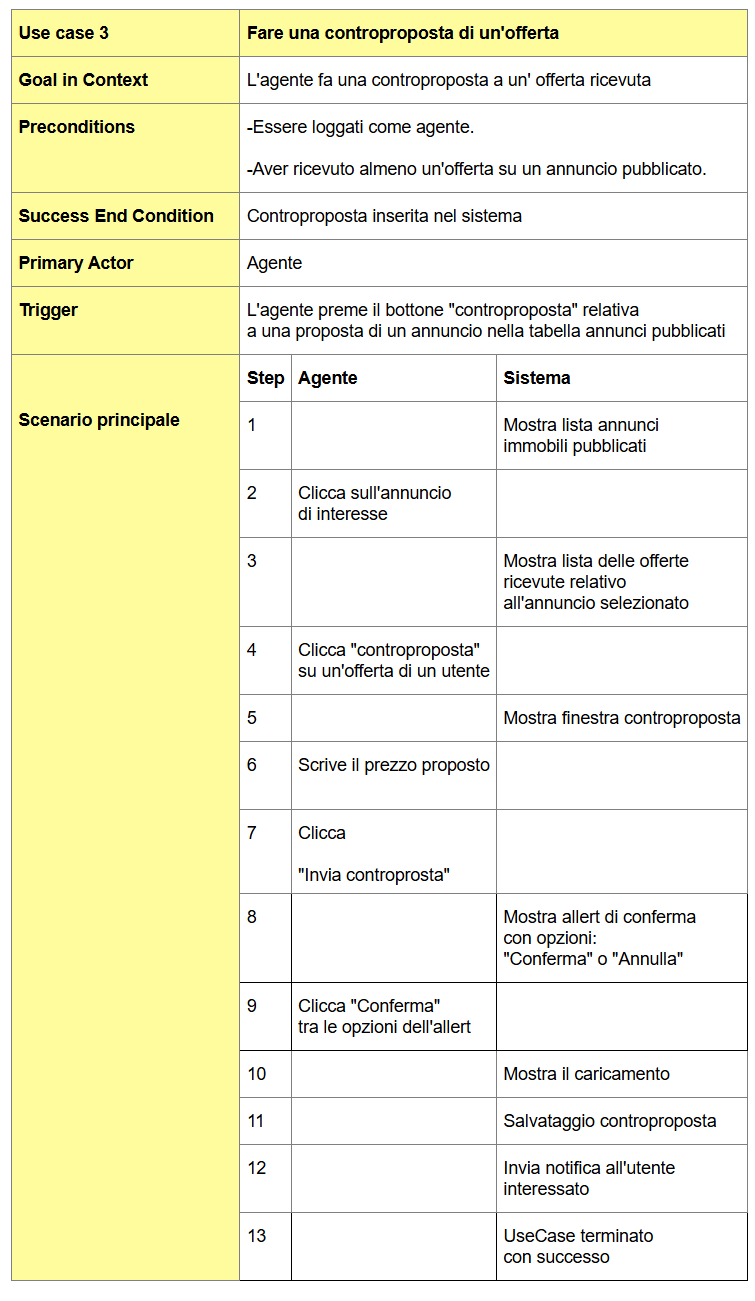
\includegraphics[width=0.8\linewidth]{"Immagini/cockburn/controproposta principale.png"}
	\caption[CockBurn extensions: registra nuovo agente]{}
	\label{fig:controproposta-principale}
\end{figure}

\newpage

\begin{figure}[H]
	\centering
	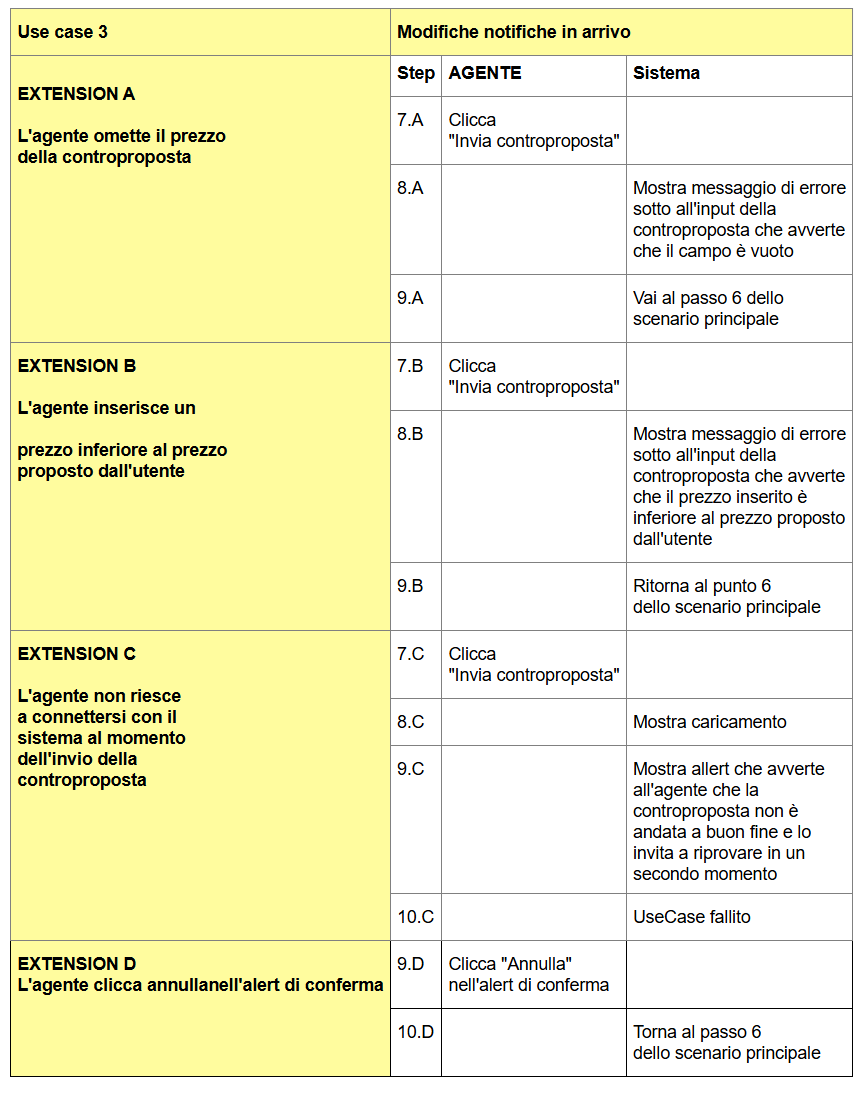
\includegraphics[width=1\linewidth]{"Immagini/cockburn/controproposta estensioni.png"}
	\caption[CockBurn extensions: registra nuovo agente]{}
	\label{fig:controproposta-estensioni}
\end{figure}
\newpage
\subsection{Cockburn: Registra nuovo agente} 

\begin{table}[H]
	\begin{tabular}{|
			>{\columncolor[HTML]{9AFF99}}l |lll|}
		\hline
		\textbf{Use case 4}                                            & \multicolumn{3}{l|}{\cellcolor[HTML]{9AFF99}\textbf{Registra nuovo agente}}                                                                                                                                                                                           \\ \hline
		Goal in Context                                                & \multicolumn{3}{l|}{Inserire un nuovo agente di un agenzia immobiliare nel sistema.}                                                                                                                                                                                  \\ \hline
		Preconditions                                                  & \multicolumn{3}{l|}{\begin{tabular}[c]{@{}l@{}}-Essere loggati come agente.\\ \\ -Aver ricevuto almeno un offerta su un \\ immobile pubblicato.\end{tabular}}                                                                                                         \\ \hline
		Success End Condition                                          & \multicolumn{3}{l|}{Salvataggio di un nuovo agente nel sistema con credenziali di default.}                                                                                                                                                                           \\ \hline
		DESCRIPTION                                                    & \multicolumn{1}{l|}{\textbf{Step}} & \multicolumn{1}{l|}{\textbf{Manager}}                                                                          & \textbf{Sistema}                                                                                                \\ \hline
		\cellcolor[HTML]{9AFF99}                                       & \multicolumn{1}{l|}{1}             & \multicolumn{1}{l|}{\begin{tabular}[c]{@{}l@{}}Clicca \\ “Registra nuovo dipendente”\end{tabular}}             &                                                                                                                 \\ \cline{2-4} 
		\cellcolor[HTML]{9AFF99}                                       & \multicolumn{1}{l|}{2}             & \multicolumn{1}{l|}{}                                                                                          & \begin{tabular}[c]{@{}l@{}}Mostra pagina \\ registrazione dipendente\end{tabular}                               \\ \cline{2-4} 
		\cellcolor[HTML]{9AFF99}                                       & \multicolumn{1}{l|}{3}             & \multicolumn{1}{l|}{\begin{tabular}[c]{@{}l@{}}Compila form\\ selezionando "Agente"\\ come ruolo\end{tabular}} &                                                                                                                 \\ \cline{2-4} 
		\cellcolor[HTML]{9AFF99}                                       & \multicolumn{1}{l|}{4}             & \multicolumn{1}{l|}{Clicca "Registra dipendente"}                                                              &                                                                                                                 \\ \cline{2-4} 
		\cellcolor[HTML]{9AFF99}                                       & \multicolumn{1}{l|}{5}             & \multicolumn{1}{l|}{}                                                                                          & \begin{tabular}[c]{@{}l@{}}Mostra allert di conferma\\ con opzioni\\ "Annulla" e "Conferma"\end{tabular}        \\ \cline{2-4} 
		\cellcolor[HTML]{9AFF99}                                       & \multicolumn{1}{l|}{6}             & \multicolumn{1}{l|}{Clicca "Conferma"}                                                                         &                                                                                                                 \\ \cline{2-4} 
		\cellcolor[HTML]{9AFF99}                                       & \multicolumn{1}{l|}{7}             & \multicolumn{1}{l|}{}                                                                                          & Mostra caricamento                                                                                              \\ \cline{2-4} 
		\cellcolor[HTML]{9AFF99}                                       & \multicolumn{1}{l|}{8}             & \multicolumn{1}{l|}{}                                                                                          & Genera credenziali di default                                                                                   \\ \cline{2-4} 
		\cellcolor[HTML]{9AFF99}                                       & \multicolumn{1}{l|}{9}             & \multicolumn{1}{l|}{}                                                                                          & \begin{tabular}[c]{@{}l@{}}Salvataggio nuovo agente\\ nel sistema con\\ credenziali di default\end{tabular}     \\ \cline{2-4} 
		\cellcolor[HTML]{9AFF99}                                       & \multicolumn{1}{l|}{10}            & \multicolumn{1}{l|}{}                                                                                          & \begin{tabular}[c]{@{}l@{}}Mostra messaggio di conferma\\ con allegato le credenziali di\\ default\end{tabular} \\ \cline{2-4} 
		\multirow{-11}{*}{\cellcolor[HTML]{9AFF99}Scenario principale} & \multicolumn{1}{l|}{11}            & \multicolumn{1}{l|}{}                                                                                          & \begin{tabular}[c]{@{}l@{}}Use case terminato\\ con successo\end{tabular}                                       \\ \hline
	\end{tabular}
\end{table}

\newpage

\begin{table}[H]
	\begin{tabular}{
			>{\columncolor[HTML]{9AFF99}}l lll}
		\hline
		\textbf{Use case 4}                                                                                                                                                                                                                                                                                 & \multicolumn{3}{l}{\cellcolor[HTML]{9AFF99}\textbf{Registra nuovo agente}}                                                                                                                                                                   \\ \hline
		\multicolumn{1}{|l|}{\cellcolor[HTML]{9AFF99}}                                                                                                                                                                                                                                                      & \multicolumn{1}{l|}{\textbf{Step}} & \multicolumn{1}{l|}{\textbf{Manager}}              & \multicolumn{1}{l|}{\textbf{Sistema}}                                                                                                              \\ \cline{2-4} 
		\multicolumn{1}{|l|}{\cellcolor[HTML]{9AFF99}}                                                                                                                                                                                                                                                      & \multicolumn{1}{l|}{4.A}           & \multicolumn{1}{l|}{Clicca  “Registra dipendente”} & \multicolumn{1}{l|}{}                                                                                                                              \\ \cline{2-4} 
		\multicolumn{1}{|l|}{\cellcolor[HTML]{9AFF99}}                                                                                                                                                                                                                                                      & \multicolumn{1}{l|}{5.A}           & \multicolumn{1}{l|}{}                              & \multicolumn{1}{l|}{\begin{tabular}[c]{@{}l@{}}Mostra errori \\ nei campi non\\ compilati correttamente\end{tabular}}                              \\ \cline{2-4} 
		\multicolumn{1}{|l|}{\multirow{-4}{*}{\cellcolor[HTML]{9AFF99}\textbf{\begin{tabular}[c]{@{}l@{}}EXTENSION A\\ \\ Non tutti i campi\\ sono compilati\\ oppure compilati\\ correttamente\end{tabular}}}}                                                                                             & \multicolumn{1}{l|}{6.A}           & \multicolumn{1}{l|}{}                              & \multicolumn{1}{l|}{\begin{tabular}[c]{@{}l@{}}Ritorna al passo 3 dello\\ scenario principale\end{tabular}}                                        \\ \hline
		\multicolumn{1}{|l|}{\cellcolor[HTML]{9AFF99}{\color[HTML]{000000} }}                                                                                                                                                                                                                               & \multicolumn{1}{l|}{6.B}           & \multicolumn{1}{l|}{Clicca "Conferma"}             & \multicolumn{1}{l|}{}                                                                                                                              \\ \cline{2-4} 
		\multicolumn{1}{|l|}{\cellcolor[HTML]{9AFF99}{\color[HTML]{000000} }}                                                                                                                                                                                                                               & \multicolumn{1}{l|}{7.B}           & \multicolumn{1}{l|}{}                              & \multicolumn{1}{l|}{Mostra caricamento}                                                                                                            \\ \cline{2-4} 
		\multicolumn{1}{|l|}{\cellcolor[HTML]{9AFF99}{\color[HTML]{000000} }}                                                                                                                                                                                                                               & \multicolumn{1}{l|}{8.B}           & \multicolumn{1}{l|}{}                              & \multicolumn{1}{l|}{\begin{tabular}[c]{@{}l@{}}Il sistema genera automaticamente\\ un email alternativa che aggiunge\\ un id univoco\end{tabular}} \\ \cline{2-4} 
		\multicolumn{1}{|l|}{\multirow{-4}{*}{\cellcolor[HTML]{9AFF99}{\color[HTML]{000000} \textbf{\begin{tabular}[c]{@{}l@{}}EXTENSION B\\ \\ Il manager tenta\\ di registrare un\\ agente il cui nome\\ e cognome sono\\ in comune con\\ un altro agente già\\ registato nel \\ sistema\end{tabular}}}}} & \multicolumn{1}{l|}{9.B}           & \multicolumn{1}{l|}{}                              & \multicolumn{1}{l|}{\begin{tabular}[c]{@{}l@{}}Ritorna al passo 9 dello\\ scenario principale\end{tabular}}                                        \\ \hline
		\multicolumn{1}{|l|}{\cellcolor[HTML]{9AFF99}}                                                                                                                                                                                                                                                      & \multicolumn{1}{l|}{6.C}           & \multicolumn{1}{l|}{Clicca "Annulla"}              & \multicolumn{1}{l|}{}                                                                                                                              \\ \cline{2-4} 
		\multicolumn{1}{|l|}{\multirow{-2}{*}{\cellcolor[HTML]{9AFF99}\textbf{\begin{tabular}[c]{@{}l@{}}EXTENSION C\\ \\ Clicca "Annulla"\\ invece di\\ "Conferma" nell'\\ allert di conferma\end{tabular}}}}                                                                                              & \multicolumn{1}{l|}{7.C}           & \multicolumn{1}{l|}{}                              & \multicolumn{1}{l|}{\begin{tabular}[c]{@{}l@{}}Ritorna al passo 3 dello\\ scenario principale\end{tabular}}                                        \\ \hline
		\multicolumn{1}{|l|}{\cellcolor[HTML]{9AFF99}}                                                                                                                                                                                                                                                      & \multicolumn{1}{l|}{6.D}           & \multicolumn{1}{l|}{Clicca "Conferma"}             & \multicolumn{1}{l|}{}                                                                                                                              \\ \cline{2-4} 
		\multicolumn{1}{|l|}{\cellcolor[HTML]{9AFF99}}                                                                                                                                                                                                                                                      & \multicolumn{1}{l|}{7.D}           & \multicolumn{1}{l|}{}                              & \multicolumn{1}{l|}{Mostra caricamento}                                                                                                            \\ \cline{2-4} 
		\multicolumn{1}{|l|}{\cellcolor[HTML]{9AFF99}}                                                                                                                                                                                                                                                      & \multicolumn{1}{l|}{8.D}           & \multicolumn{1}{l|}{}                              & \multicolumn{1}{l|}{\begin{tabular}[c]{@{}l@{}}Avvisa l'utente dell'operazione\\ fallita per motivi tecnici\end{tabular}}                          \\ \cline{2-4} 
		\multicolumn{1}{|l|}{\multirow{-4}{*}{\cellcolor[HTML]{9AFF99}\textbf{\begin{tabular}[c]{@{}l@{}}EXTENSION D\\ \\ L'utente non \\ riesce a connettersi\\ con il sistema\end{tabular}}}}                                                                                                             & 9.D                                &                                                    & User case fallito                                                                                                                                  \\ \hline
	\end{tabular}
\end{table}